\documentclass{bioinfo}
\copyrightyear{2019} \pubyear{2019}

\access{Advance Access Publication Date: 27 June 2019}
\appnotes{Data and text mining}
\usepackage{textcomp}
\usepackage{booktabs}
\usepackage[table,xcdraw]{xcolor}
\bibliographystyle{unsrt}

\begin{document}


\firstpage{1}

\subtitle{Data and text mining}

\title[I2EHR: Interactive Integrated Electronic Health Records]{I2EHR: Interactive Integrated Electronic Health Records}
\author[Sample \textit{et~al}.]{Shane Crinion\,$^{\text{\sfb}*}$, Pilib \'{O} Broin\,}
\address{$^{\text{\sf 1}}$School of Mathematics, Statistics \& Applied Mathematics, National University of Ireland, Galway, H91 H3CY\\}

\corresp{$^\ast$To whom correspondence should be addressed.}

\history{Received on XXXXX; revised on XXXXX; accepted on XXXXX}

\editor{Associate Editor: XXXXXXX}

\abstract{\textbf{Motivation:} Electronic health records contain dense, longitudinal data that cannot be used to full potential due to a lack of standardisation and infrastructure. A framework that allows integrative analysis of clinical and genomic data is likely to improve healthcare delivery and predictive analytics. 
\\
\textbf{Summary:} We present the Interactive Integrated Electronic Health Record (I2EHR), a dashboard built using R/Shiny allowing integrative patient and cohort analysis across operating systems. The interface allows the user to view patient or cohort level and generate visualisations based on user-selected measurements. This model, generated using realistic synthetic clinical data, is then integrated with gene expression profiles to develop a realistic and longitudinal model of disease pathology. Lastly, the model uses the newly identified genotype-phenotype associations to perform predictive modelling. 
\\
\textbf{Availability:} I2EHR can be obtained from GitHub:  {\tt \small github.com\slash shanecrinion\slash I2EHR}. The subdirectory ``I2EHR\textunderscore APP" contains the application script and clinical data files. The genomic data is downloaded within the script from the Gene Expression Omnibus and is accessible under the accession number GSE46097.
\\
\textbf{Contact:} {s.crinion1@nuigalway.ie} 
\\
\textbf{Supplementary information:} Supplementary data is available from the Supplementary Information file on the I2EHR online repository.}


\maketitle
\section{Introduction}
The widespread implementation of the electronic health record (EHR) substantially improves the quality and efficiency of healthcare service delivery \cite{Evans2016}. By using EHR systems, an extensive and longitudinal profile of the patient's historical recordings can be built at the point of care. Substantial improvements to healthcare delivery and research can occur following integration of EHR systems; the use of digital records in healthcare has significantly reduced errors and increases the amount of usable data for clinical research \citep{Williams2019}. 
Advanced EHR systems that enable clinical decision support (CDS) are used for decision making, forecasting patient outcomes and modifying treatment promptly to improve delivery of diagnosis and drug prescription \citep{CDS2}.
Given the exponentially growing size of clinical and genomic data available, the EHR provides a storage method beyond human capacity \cite{Williams2019}. Data stored in EHRs including vital signs, billing data, laboratory results or genomic data in the most advanced systems \citep{Denny2012}.      

However, the most useful function with EHR data may be the potential for text mining with patient data. Longitudinal, dense patient data stored within EHRs is especially useful for understanding disease epidemiology and progression \citep{Casey2016}. Providing access to high quality lifetime patient data is extremely useful for improving treatment of complex, heterogeneous diseases \citep{Faria-Campos2015} including type 2 diabetes (T2D) and cancer. 


The user interface (UI) of EHRs is commonly designed poorly and many lack the functionality to view numerous clinical recordings simultaneously \cite{Menachemi2011}. At patient level, a timeline or other visual representation may improve understanding of changes in patient health over time. Risk factors that signal disease progression for example, high BMI in T2D or high blood pressure in cardiovascular disease (CVD), may show up that are not obvious with static data.

Time-based visualisations can also identify novel risk factors that may not be obvious throughout disease progression. Identifying new links between clinical measurements and patient outcome could be used to improve prognosis prediction or CDS functionality such as drug selection based on disease severity. However, the potential for a clinician to find new links or assess patient health recordings is greatly limited by the need to manually examine changes. Improving the digital readability of clinical data increases the data research potential as large cohorts can be built and studied. Researchers can use structured clinical data to study changes in the cohort's clinical recordings due to deterioration in health or drug prescription. For example, a cohort of opioid addicts accessed through EHR data would be useful for identifying changes due to drug use or warning signs associated with death \citep{Casey2016}. 


In order for clinical data to be integrative, numerous challenges need to be addressed including the lack of standardisation in data format. The development of integrative tools in healthcare has been limited by the wide variety of healthcare data available, causing reduced ability to process patient information and a lack of software for data analysis \citep{Evans2016}.  Concerns regarding privacy of sensitive patient data further exasperates the lack of medical software \cite{Ross2014}. The use of personal patient information requires that prior consent and adherence to legal and technical protections are followed which can result in delayed or restricted processing of patient data. 


Approaches to improve health informatics have addressed the data entry format, the interactivity of the data format and the availability of test data. HL7 Fast Healthcare Interoperability Resources (FHIR) \cite{Hong2017}  is a clinical data standard that provides a framework to improve data entry and subsequently increase the interoperability and potential for data exchange between EHRs. ShinyFHIR is an application that allows interaction with FHIR-based data and demonstrates how standardised data can be used the enhance clinical analysis \cite{Hong2017}. 
The ShinyFHIR approach demonstrates the suitability of the FHIR approach to work for numerous servers and across platforms for clinical data analysis using the \textit{R} and \textit{Shiny} packages. Synthea is an appraoch that address the lack of available clinical data by producing synthetic but realistic EHR data that can be used for medical software development \citep{Synthea}. Usage of diagnosis codes have also improved standardisation and allowed the improved exchange of notes between departments. Using diagnostic codes also improves computational readability and subsequently facilitates machine learning approaches for improved prediction of disease progression and treatment plan selection. 

The integration of genomic data to EHRs (such as in biobanks) have been shown have huge innovative potential and potential to improve clinical research \citep{Denny2012}. However, a lack standardisation of clinical data format also limits the potential for genomic data integration. Many limitations exist which prevent the integration of genomic data into genomic health records; one example is the lack of training or knowledge in genomic analysis result can result in poor interpretation of genetic variations and significance levels in disease diagnosis \citep{Fein2014}.  


To address current challenges associated with the integration of clinical and genomic data, we designed a model to integrate data and provide visual and timeline representations of patient recordings. As outlined in Figure 1, the aims of this project include (a) to develop a dashboard to integrate clinical and genomic data (b) create simple predictive analytics using the patient and clinical data and (c) use GEO to integrate gene expression profiles and provide proof-of-concept for combined clinical and molecular analytics. 

Given the increasing ease and widespread use of genomic analysis, this approach could be applied to many hospital EHRs to provide useful statistical results for genomic research. The tool requires little expertise to use and can be deployed to all devices with little to no configuration. By providing an integrated system containing combined analytics for clinical and genomic data, we aim to improve the accessibility of combined analytics at patient or cohort level and further improve the utilisation of big data in genomics. 


%\enlargethispage{12pt}
\begin{methods}
\section{Materials and Methods}
\begin{figure}
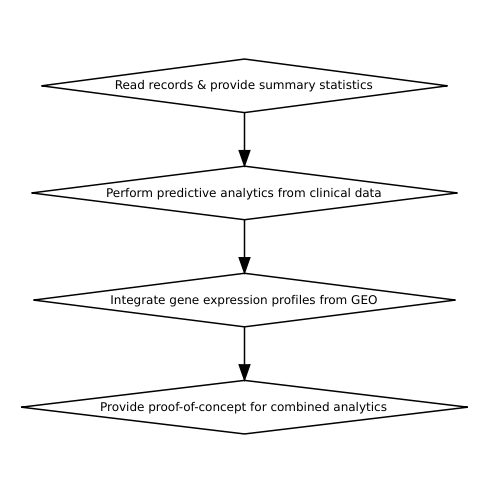
\includegraphics[width=8cm, height=11cm]{/media/shane/Data/github/I2EHR/I2EHR_APP/www/flowchart.png}
\caption{Analysis flowchart: Clinical data is read, analysed and integrated with genomic data. Clinical observations are then integrated with genomic expression values to visualise subgroup variation.}
\end{figure}

In order to develop the integrative application, the clinical data came from Synthea \citep{Synthea}, a package used to generate synthetic, realistic EHR data. Synthea was developed due to the lack of clinical data available for use in software development and other research or education purposes without any concerns for legal, privacy or security issues \cite{Synthea}. The package also follows the standardised FHIR HL7 format and provides a source of `clean' structured data which contains no discrepancies due to human error. Synthea is built with the top-down approach named Publicly Available Data Approach to the Realistic Synthetic EHR (PADASER) which is a framework to generate EHR data coded in the HL7 FHIR format. The PADASER framework uses publicly available datasets to populate synthetic EHR including health incidence statistics, clinical practise guidelines (CPGs) and Protocols and Medical Coding Dictionaries. The approach has a core principal of privacy and avoids any risk of patient re-identification as reported in previous studies \citep{ElEmam2011}.  

At the core level, Synthea consists of various generic modules to model the 10 most common reasons for patient visits in the United States according to the Global Burden of Disease \citep{Synthea}. The patients generated were from the `Cardiovascular Disease' module which consists of coronary heart disease, myocardial infarction, cardiac arrest, stroke and atrial fibrillation. The `wellness' module was also used which contains clinical measurements such as body mass index (BMI), diastolic blood pressure and pain severity which can be useful for visualising change over time. 

The original population generated consisted of 1000 patients originating from Boston, MA. The output consists of eleven CSV files containing various types of clinical data namely allergies, careplans, conditions, encounters, imaging studies, immunizations, medications, observations, organizations, procedures and providers. Each file contains clinical information for patients using their patient ID number. The patients file contains demographic information such as patient ID, first name, last name, address, gender, ethnicity and race (figure 3). The conditions file includes the associated condition for the patient (for example coronary heart disease for patient 1e48d3da-d4f0-4680-8106-2304c9d1426e). The encounters file records each patient encounter, all of which are under "Encounter for check up (procedure)" or "Emergency Encounter". The observations file contains every clinical measurement for the patient generated from the wellness module such as BMI and diastolic blood pressure. The procedures indicates the treatment provided for the patient, for example "electrical cardioversion" and "Catheter ablation of tissue of heart". The population had no generated information for  allergies, careplans, imaging studies or providers. The data contained within each file was used to build a longitudinal patient profile and to differentiate subgroups within the cohort.


Measurements extracted from the observations file were selected to model the time dependant variation of patient 

Clinical measurements from the observations file were selected to model the variation expected for a cardiovascular disease patient. BMI, diastolic blood pressure and systolic blood pressure were selected as the outcomes of interest for subgroup selection. A BMI measurement of above 30 is considered high and is expected for an individual with a cardiovascular disease \cite{Ellsworth2014}. Similarly, the diastolic and systolic blood pressure measurements are expectedly elevated in a cardiovascular disease patient and measured above 80 and 120 mm Hg respectively \cite{Ellsworth2014}.   
These measurements are recorded in table 1. 



% Please add the following required packages to your document preamble:
% \usepackage{booktabs}

\begin{table}[]
\begin{tabular}{@{}llll@{}}
\toprule
\rowcolor[HTML]{EFEFEF} 
\textbf{Observation (units)} & \textbf{Data Source} & \textbf{Normal Level} & \textbf{CVD Level} \\ \midrule
BMI                          & Clinical             & \textless 30          & \textgreater 30    \\
Diabetes (mmol/L)            & Genomic              & \textgreater 5.6      & \textgreater{}=7   \\
Diastolic BP (mm Hg)         & Clinical             & \textless 80          & \textgreater 80    \\
Systolic BP (mm Hg)          & Clinical             & \textless 120         & \textgreater 120   \\ \bottomrule
\figure{Each of the }
\end{tabular}
\end{table}


The aims of this project include integration of clinical data with gene expression profiles to allow combined clinical / molecular analytics. Gene expression profiles were sourced from the Gene Expression Omnibus data repository which contains many publicly genomic data sets including expression by array sets. \textit{"Expression data of Participants of Ornish intervention and Control group"} was selected, a study that aimed to examine the impact of a CVD risk reduction program on peripheral blood gene expression profiles in 63 Caucasian participants and 63 matched controls following rigorous lifestyle modification and identify regulatory pathways associated with cardiovascular health. Entry criteria for the  at-risk participants included diagnosis of coronary artery disease (CAD) and diagnosis of diabetes. Controls were matched based on age, sex and disease status. The number of participants with diabetes and CAD was matched with controls and consisted of 10 diabetes and 23 CAD samples each. 

The expression data consists of 379 CEL files with 3 samples for each individual taken at baseline, 3 months and 1 year. Genotyping was performed using [\ HG-U133A\textunderscore 2 ]\ Affymetrix Human Genome U133A 2.0 Array. The data was background corrected using robust multi-array average (RMA) and log2 transformed prior to integration. The data was extracted GEOquery, a Bioconductor package that facilitates import of microarray data directly from R using the GEO accession number \cite{Davis2007}. The command {\tt \small getGEO("GSE46097")} imports the data as an ExpressionSet object which combines the sample phenotypic data and experimental chip and technology data used for the experiment. The function {\tt \small exprs} is used to extract the per probe expression levels. 


To integrate the clinical and genomic data, each sample from the generated Synthea data was assigned a GEO accession corresponding with a case or control sample. Each sample within the genomic data was subsequently assigned a patient ID. Given that Synthea does not allow control sample generation, the conditions file was manipulated to label the control patient's condition accordingly. The clinical observations values for BMI, diastolic blood pressure and systolic blood pressure were categorised based on the thresholds within table one. For the participant vs. control relative log expresssion plot (RLE), the associated control was not labelled as such. A control was selected by subsetting to samples that was within five years of age with matching diabetes status, CAD status and gender. Additionally, the genomic data was subset to baseline and 1 year samples only for the t-test step within the patient level clinical analysis.


The development of this dashboard was made possible using the packages R and shiny 
R version 3.6.0. The user can obtain the app from {\tt \small github.com/shanecrinion/I2EHR/I2EHR\textunderscore APP.}  The front-end packages used for app development included the following: shinydashboard and shinywidgets. Visualisations were generated using the ggplot2 and plotly packages. Associated packages include: ggridges, lattice, viridis, DiagrammeR, gplots, ggplot2, geneplotter, RColorBrewer and pheatmap. The integration and analysis of genomic data was made possible using multiple packages from Bioconductor which include GEOquery, oligo, arrayQualityMetrics and the analytics and statistics packages limma, topGO, ReactomePA and clusterProfiler. 


\end{methods}




\section{Results}
I2EHR contains 6 major components that were deemed most relevant for the integrated analysis of the data: (1) patient level data query 
(2) patient level genomic analysis 
(3) cohort level observations plot 
(4) principal component analysis 
(5) subgroup expression analysis 
(6) differential expression analysis



\subsection{Patient level data query}
\begin{figure}[!h]
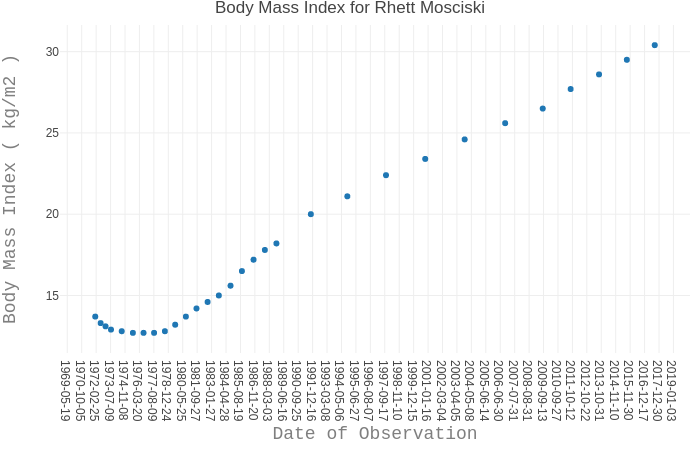
\includegraphics[width=8cm]{BMIpatient.png}
\caption{Observation plot: The x-axis indicates the date of observation and y-axis indicates the measurement. A drop down menu allows selection of the observation to observe over time.}
\end{figure}

To query a patient, select the "Patient Analysis" tab and enter the patient ID number in the search bar. A table including the patient ID, full name, gender, ethnicity and race is generated. 
To query an observation, select a type from the drop down such as "Body Mass Index". The patient observation type and name populates a plot. The plot is generated using \textit{plotly} package which allows the user interact by zoom, pan or hover to display corresponding information for the selected data point. The name, description, units and dates are extracted to populate a unique plot for the patient/observation. Under the heading "Additional Information", a table can be generated containing all other patient recordings from of the CSV files. 



\subsection{Patient level gene expression variation}

\begin{figure}[!h]
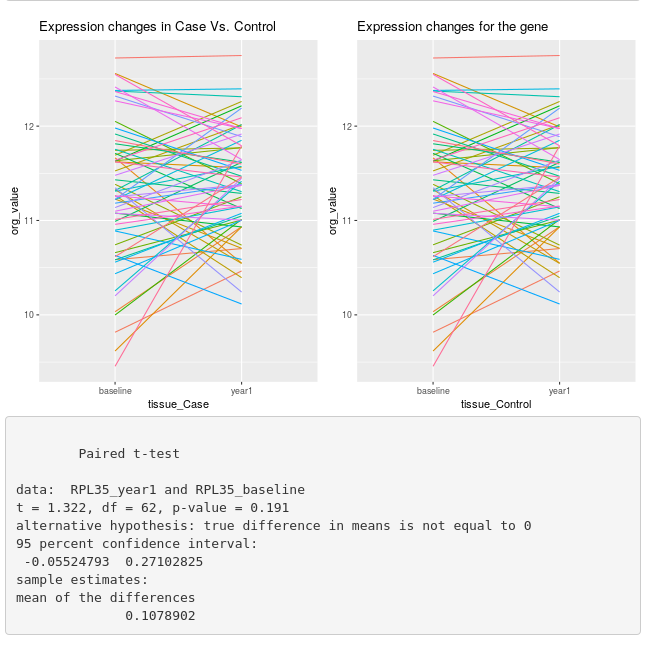
\includegraphics[width=8cm, height=8cm]{exprschangettest.png}
\caption{Expression changes: each plotted line represents an individuals variation in gene expression between baseline and 1 year assessment.}
\end{figure}

As seen in figure 3, the dashboard allows a visualisation of patient level gene expression variation. A table of the plot contains all genes and probe information; this can be used to select a probe and view gene expression changes in the case and control. Additionally, a t-test is generated below indicating the significance of the case and control samples variation.


\subsection{Cohort level barcharts}
\begin{figure}[!h]
\center
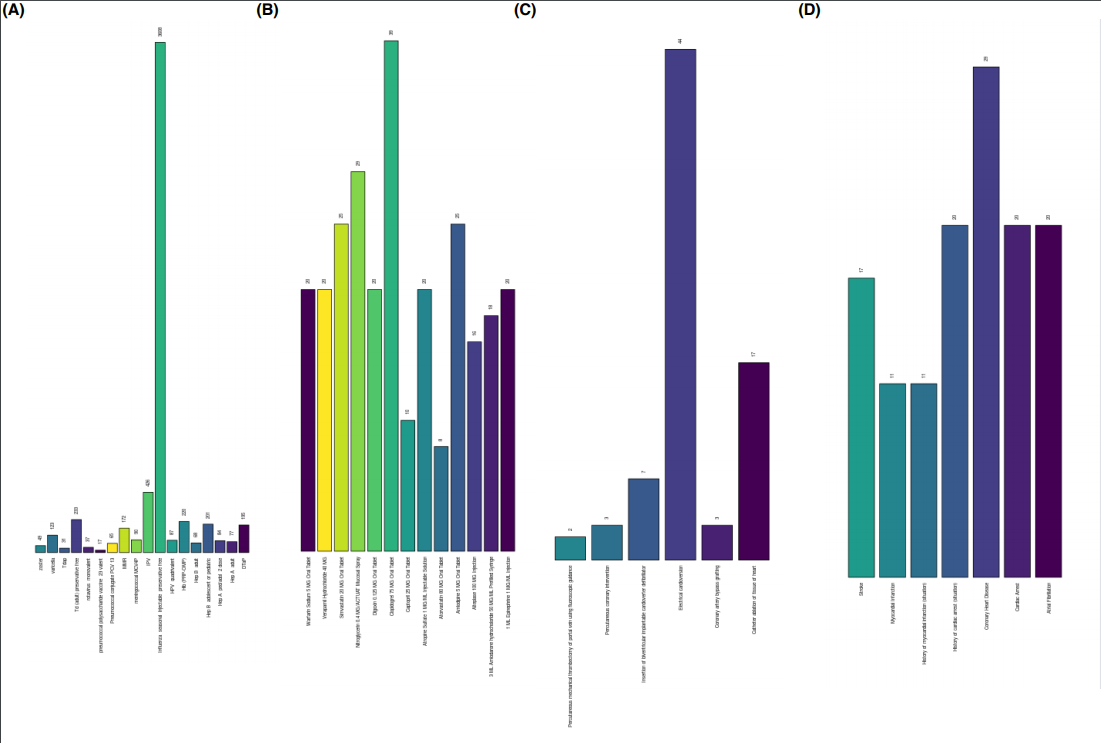
\includegraphics[width=8cm]{barcharts.png}
\caption{Barcharts: Plots indicate the frequency for each of (A) immunizations, (B) medications, (C) procedures and (D) conditions at cohort level.} 
\end{figure}

Cohort level barcharts are available within the `Cohort' section on the dashboard sidebar.
As seen in Figure 4, barcharts are used to visualise the dispersal of clinical entries for the cohort. Buttons allow the user to select between viewing frequency of recordings for immunizations, medications, procedures and conditions. This can be used to understand the most common diseases or treatments being applied for the cohort.  


\begin{figure*}[!t]
\center
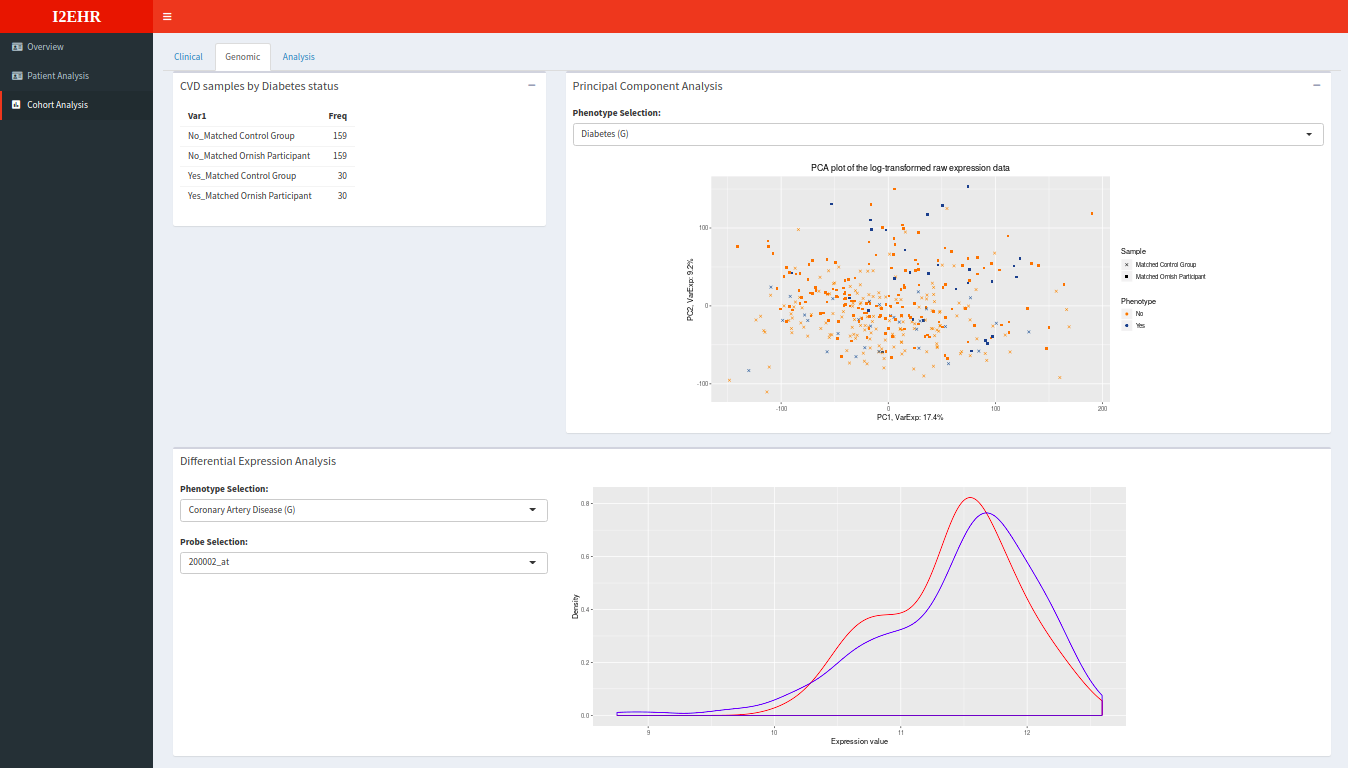
\includegraphics[width=17cm]{DashboardLayout2.png}
\caption{Dashboard Layout: I2EHR UI including the PCA and density plots allowing subgroup selection. This can be used to identify subgroup clustering or gene expression variation.} 
\end{figure*}

\subsection{Principal component analysis}

Principal component analysis (PCA) is used to identify possibly correlated variables and visualise genetic distance. The PCA plot of Figure 5 demonstrates the integration of clinical and genomic variables. The user selects the colour fill of the PCA from the three clinical data measurements (BMI, SBP and DBP) and two genomic data measurements (diabetes and CAD status). 



\subsection{Gene expression density plots}
\begin{figure}[!h]
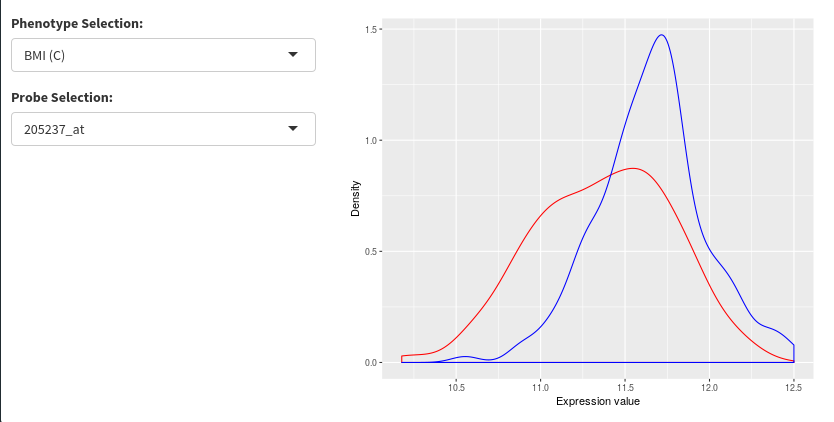
\includegraphics[width=8cm, height=8cm]{densityplot.png}
\caption{Density plots: The generated plots indicate the gene expression variation found between the participant (blue) and control (red).}
\end{figure}


The gene expression density plots can be used to identify the genomic variation between the subgroups. The user selects the probe and subgroup to display. The table below the density plot can be used to select an associated probe for the gene of interest. The plots indicate the level of expression found within the two subgroups. This information can be used to identify if a gene is over or under expressed in a certain cohort subgroup.

\subsection{Microarray analysis}

Given the integrative design of the application, the differential expression analysis steps of the microarray analysis steps are contained within the "Analysis" tab of the "Cohort Analysis" section of the dashboard to provide an all-in-one integrative research application. This can be used to identify gene ontologies for further analysis within the integrated subgroups.
Top gene ontologies can be useful when researching the genes to compare within newly identified subgroups using the application. 

The microarray analysis follows standard procedure of quality control, normalisation, differential expression analysis and biological interpretation. The genomic data in this study indicated that normalisation and quality control was already performed. After confirming this, these results were not included in the application and can be found in the supplementary information. The quality control includes a number of visualisations for identifying probe level variation and ensuring no sample reading is an outlier such as the between array comparison, array intensity distribution, variance, standard deviation from the mean and individual array quality. Normalisation of data was performed using the ‘Robust Multi-Array Average (RMA) method and the oligo package prior to integration.

The next tab, differential expression analysis, is used to identify the variation due to the risk factor. The log2 fold change and multiple testing correction is performed using ‘limma` on Expression Atlas data. The interpretation is through heatmaps, functional annotation and network analysis. This can then be used to identify the sample relationships and the genes that are associated with the disease in question.



\begin{Discussion}

\section{Discussion}
\enlargethispage{6pt}
The motivation for the study was to develop a framework that integrated both clinical and genomic data; this framework was generated due to lack of a similar system and the potential benefits for identifying new patterns in clinical subgroups based on genomic expression patterns. I2EHR demonstrates data collected in FHIR format can be integrated for exploratory purposes and integrated with genomic data on a single and easy-to-use usable platform.

Visualisations of longitudinal clinical data proved useful for identifying changes over time associated with cardiovascular disorders. I2EHR facilitates further identification of new risk factors for disease progression by plotting observations on a patient or cohort basis. Longitudinal plots can identify high risk patients and has the potential to facilitate new clinical warning signs. By visualizing the healthcare data using dashboards, patient stratification is accelerated and the trends in patient health can be used to for faster intervention and improved understanding of the disease pathology. The graphical representation of the data results in faster diagnosis and improved healthcare by allowing the development of predictive models and risk estimation with an easy, accessible interface.  


Issues regarding standardisation have caused difficultly in the adoption of plots and other visualisation aids. Heterogenous, complex data 
within current EHRs due to a lack of clinical data entry standards have greatly reduced the ability to integrate genomic data. In the absence of standardised methods such as FHIR, structuring clinical observations in according with gene expression profiles is difficult. This dashboard provides an example of clinical and genomic data integration that can be applied to data structured in FHIR format.


Normally EHRs platforms do not support simultaneous view of the clinical data entries with genomic data. I2EHR allows the user to view their data entries in table format or view the  clinical observations using the plotly generated plots. A core element for widespread implementation is ease of use; presented here is a dashboard interface allowing easy access and interactivity for the user. The user can view clinical observations, genomic expression profiles and differential expression analysis results together. Providing a simple dashboard that requires little expertise and quick visualisation of these patterns will improve the adoption of integrated approaches such as I2EHR.


Several limitations must be addressed regarding Synthea including the synthetic nature of the data. Synthea developers indicate that the data is useful for IT developments however the clinical observations and statistics should not be considered usable for identification of disease patterns. No clinical decision making should be performed using the data and use should be for proof of purpose only. There are minor issues regarding the categorisation of disease for example entries named `History of myocardial infarction (situation)' and 'myocardial infarction' are the same but fall under different categorisation. Synthea also contains discrepancies with demographic data statistics that have been addressed in the issues section of their GitHub account and in other reviews. Synthea developers are continuously improving the data to stay up to date. 

Another caveat using Synthea occurs when generating control samples. As all samples available are disease patients, each individual was diagnosed with a disease from the CVD module. Synthea does not allow the generation of control patients which required manual manipulation and subsequently may cause discrepancies when comparing results from this analysis with real cases. 

Despite the caveats, Synthea has proved highly useful for the objectives of the project. Synthea improved efficiency by allowing instant data usage and manipulation for effective modelling of a CVD cohort. This has also eliminated time associated with data cleaning given that clinical data is often ‘dirty’ due to errors or non-structured data entry. Efficiency is also improved by the elimination of issues associated with privacy including de-personalising the data and requesting new data privileges.

This framework developed with the help of Synthea allows interoperability among departments and the use of clinical and genomic data for its relevant function. The use of FHIR format makes the dashboard universal for clinical data. Further emphasis on data standardisation is a core component for utilisation of I2EHR and the wider capabilities of integrated clinical and genomic research.

The use of integrative data is particularly useful for complex, polygenic diseases. This approach intends to give clinical researchers the insight required to improve treatment of heterogenous disorders and improve disease subgroup identification by facilitating integration of genomic data. Differential expression patterns can be used to personalise treatment dependant on the gene expression evident within the patient. For example, the use of visualisations such as overlapping density plots of expression values for the case and control can be used to select the correct medication to manipulate gene expression desirably. 

The extraction of data using GEO also proved to be more challenging when finding a suitable sample of gene expression data. GEO datasets that contained a large sample of gene expression data could not be found that exceeded 12 patients with diagnosis of T2D and no other disease. The alternative data repository ArrayExpress \citep{Athar2018} also showed no results for larger datasets. For this reason, a larger cardiovascular disease sample set with a subset of diabetes patients was used. Testing the application with each dataset proved useful in ensuring interoperability with other datasets stored as ExpressionSet objects. 


For application development, Shiny proved especially useful for the development of useful software for use in analysis of clinical and genomic data. Shiny allowed the development of this dashboard which will facilitate integrative analysis on a user-friendly dashboard. The primary aim of this project was to perform integrative analysis however ease of use is necessary for increased implementation. The dashboard allows overlaying of clinical and genomic data to view the gene expression pattern in relation to the clinical observations and potentially identify new associations between gene expression and clinical observations. 


To conclude, I2EHR provides a platform that can be used across platforms for the integrated analysis of clinical and genomic data. Further developments will be possible given greater adoption of a standardised data format in EHRs.


To conclude I2EHR is a dashboard that successfully demonstrates the potential for integration that is possible using standardised data format. Standardisation of data allowed the development of plots and tables useful for understanding patient health and cohort make up. The integration of clinical and genomic data has well defined potential in healthcare and research and will facilitate the discovery of new disease patterns as integration becomes more and more common. 


\end{Discussion} 


%%%%%%%%%%%%%%%%%%%%%%%%%%%%%%%%%%%%%%%%%%%%%%%%%%%%%%%%%%%%%%%%%%%%%%%%%%%%%%%%%%%%%
%
%     please remove the " % " symbol from \centerline{\includegraphics{fig01.eps}}
%     as it may ignore the figures.
%
%%%%%%%%%%%%%%%%%%%%%%%%%%%%%%%%%%%%%%%%%%%%%%%%%%%%%%%%%%%%%%%%%%%%%%%%%%%%%%%%%%%%%%


\section*{Acknowledgements}
I would like to thank Dr. Pilib \'{O} Broin for the helpful advice and guidance throughout the project. I also would like to thank the developers of R, Shiny and Synthea for their applications that allowed this development to happen.

\vspace*{-1pt}

\section*{Conflict of interest}
No conflict of interest is declared. 




\bibliographystyle{natbib}
%\bibliographystyle{achemnat}
%\bibliographystyle{plainnat}
%\bibliographystyle{abbrv}
%\bibliographystyle{bioinformatics}
%
%\bibliographystyle{plain}
%
%\bibliography{Document}

\bibliography{newref}

\end{document}
